\documentclass[useAMS,usenatbib]{mn2e}
\pdfoutput=1
\usepackage[varg]{txfonts}
\usepackage{astrojournals}
\usepackage{graphicx}
\usepackage{microtype}
\usepackage{xcolor}
\usepackage{fixltx2e}
\usepackage{hyperref}
\usepackage{siunitx}
\hypersetup{colorlinks=True, linkcolor=blue!50!black, citecolor=black,
  urlcolor=blue!50!black}

\usepackage{color}

\newcommand\texttheta{\ensuremath{\theta}}
\newcommand\thC{\texttheta\textsuperscript{1}\,Ori~C}
\newcommand\elec{\ensuremath{_{\mathrm{e}}}}
\newcommand\Ion[2]{\ensuremath{\mathrm{#1\,\scriptstyle #2}}}
\newcounter{ionstage}
\newcommand{\ion}[2]{% needs to be renewcommand with aastex
  \setcounter{ionstage}{#2}%
  \Ion{#1}{\Roman{ionstage}}}
\newcommand\nii{[\ion{N}{2}]}
\newcommand\oi{[\ion{O}{1}]}
\newcommand\ha{\ensuremath{\mathrm{H\alpha}}}
\newcommand\sii{[\ion{S}{2}]}
\newcommand\oiii{[\ion{O}{3}]}
\newcommand\hii{\ion{H}{2}}

\begin{document}

\begin{figure*}
  \setkeys{Gin}{width=\linewidth}
  \centering
  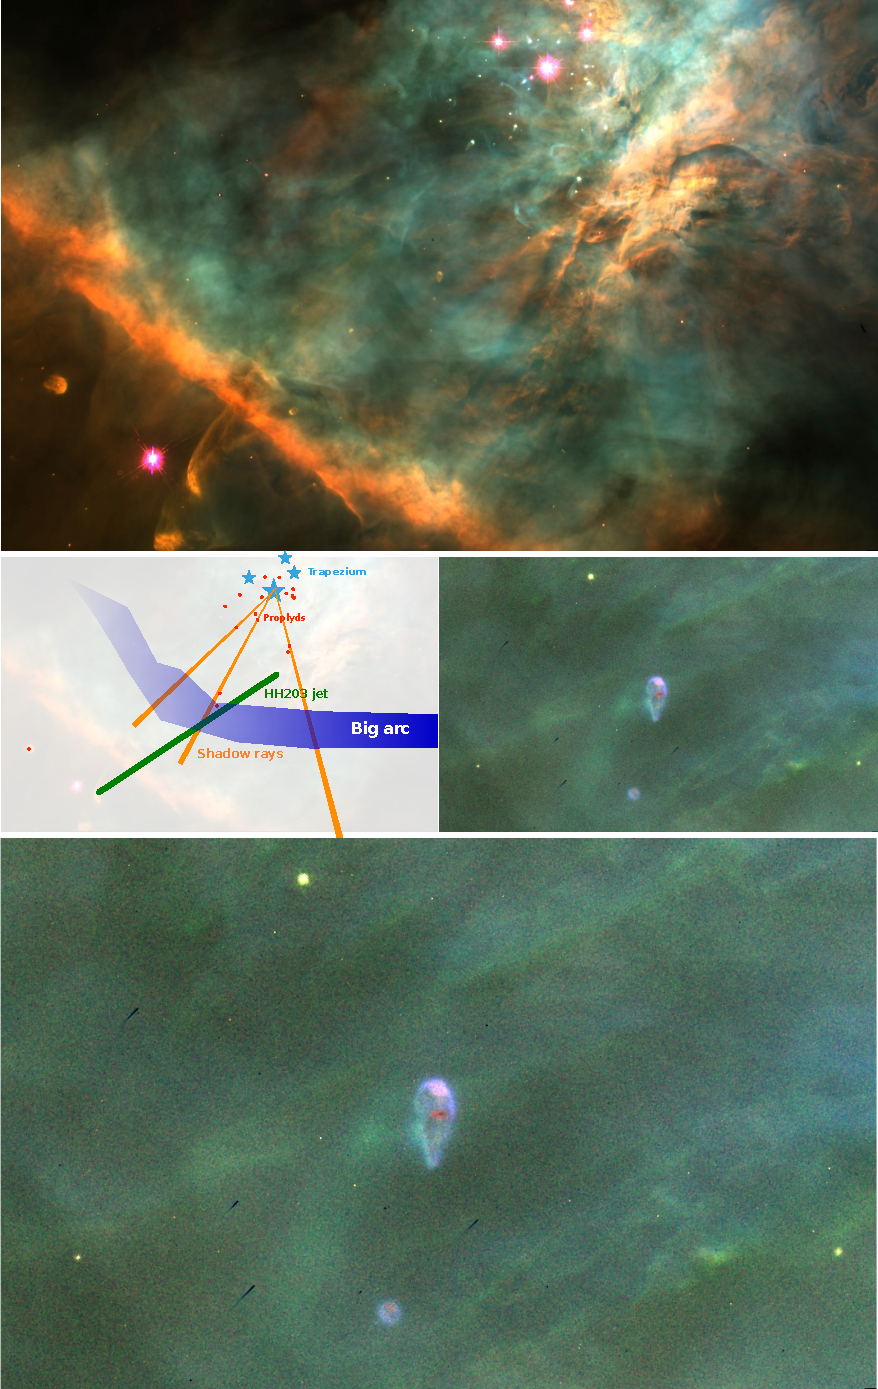
\includegraphics{hst10-environment-inkscape}
  \caption{Left panels: Large-scale view of HST~10 in the context of the Orion Nebula.  
    Three-color image in the filters of \nii{} (red), \ha{} (green), and \oiii{} (blue),
    based on a mosaic of \textit{HST} WFC observations 
    descibed in \protect\cite{1996AJ....111..846O}.  
    Right panels: Zoomed view of HST~10 and its immediate environs.
    Three-color image in the filters of \oi{} (red), \sii{} (green), and \nii{} (blue),
    based on \textit{HST} PC observations 
    described in \protect\cite{1998AJ....115..263O}.  
    The labelled objects are described in the test.
  }
  \label{fig:wfpc2-images}
\end{figure*}

\section{Introduction}

PART WRITTEN BY YIANNIS

ALTHOUGH I HAVE PUT THIS AS INTRODUCTION, YOU MIGHT FEEL IT WOULD BE BETTER IN THE DISCUSSION SECTION. 

The location on the sky of HST~10 (182-413) is halfway between 
the inner Trapezium cluster and the Bright Bar region (see Fig.~\ref{fig:wfpc2-images}), 
at an angular separation of roughly \(1'\) to the south-south-east from \thC{} (O7V), 
the principal illuminating star of the nebula.  
Kinematic studies of the emission from the proplyd \citep{1999AJ....118.2350H} 
suggest that it is situated in the foreground of the nebula, 
with a true separation from \thC{} of 0.2--0.3~pc.  
The proplyd is larger and fainter than the proplyds found close to the Trapezium, 
with a less elongated and less symmetric tail.  
This is in line with the general trends seen in the proplyds 
\citep{1998AJ....116..293B, 1998AJ....115..263O}, 
which can be understood in terms of a model whereby 
protostellar disks around the young low-mass stars in the nebula 
are evaporated by the ultraviolet radiation from the high-mass stars 
\citep{Johnstone:1998, Henney:1998}.  

Unlike in many of the smaller, brighter proplyds, 
the circumstellar disk is clearly visible in HST~10.  
In most emission lines, it is seen in absorption, 
but it is seen in emission in the H\(_2\)~2.12\(\mu\)m line \citep{1998ApJ...492L.173C} 
and in the \oi{} 6300~\AA{} line \citep{1998AJ....116..293B}. 
The \oi{} emission is shown in red in the right panel of our Figure~\ref{fig:wfpc2-images}, 
and the emission from the disk surface is believed to arise from the 
photodissociation of OH at the base of the neutral evaporated flow
\citep{Storzer:1998}.
There is also a faint high-velocity microjet detected in \oi{} \citep{1999AJ....118.2350H},
which extends perpendicular to the disk \citep{2000AJ....119.2919B}. 

Although the proplyds close to the Trapezium tend to be very symmetric 
about the line that joins them to \thC{},
this is not so true of HST~10, which seems to be governed by two different axes. 
The rotational axis of the disk and jet is oriented north-south, 
while the direction to \thC{} is at roughly \(30^\circ\) to this,
at a position angle of \(330^\circ\).  
This produces considerable distortion in the shape of the proplyd,
with the tail, in particular, seemingly more governed by the jet axis 
than the ionizing radiation field.

The Orion Nebula is highly structured at all scales 
and many previously studied nebular features pass through or near 
the immediate vicinity of HST~10, as illustrated in Figure~\ref{fig:wfpc2-images}.
The shadow rays \citep{2000AJ....119.2311O}, are low-ionization,
strictly linear features, which are seen outside the positions of some of the brighter proplyds,
and are exactly aligned with the outer projection of the line joining \thC{} and the proplyd
(see Fig.~2 of \citealt{ODell:2009a}). 
Three such rays are indicated in the Figure: the two most prominent, 
which are cast by 177-341 (HST~1) and 159-350 (HST~3), 
plus a much fainter one, which is cast by 170-337 
and which passes within \(2''\) of HST~10 in projection. 
Unlike HST~10, 170-337 shows evidence of being located behind the Trapezium stars \citep{1999AJ....118.2350H}, and therefore its shadow must be also,
so it is very unlikely to be physically close to HST~10. 
The bar features are another type of linear structure that is very common in the nebula 
\citep{2000AJ....120..382O}, of which the Bright Bar is the most prominent example. 
These are regions where the line of sight is tangential to a local ionization front, 
but the exact geometry is unclear in many cases. 
\citet{2007AJ....133..952G} found that some faint compact bars are associated with dark lanes
that are seen as linear extinction features in red-shifted velocity channels. 
Such is the case for the jagged low ionization filaments that cross the field of HST~10, 
as shown in the right panel of Figure~\ref{fig:wfpc2-images}. 
This type of emission feature may represent the ionized skin of a dense molecular filament 
that is protruding into the \hii{} region, in which case it is likely to be close to the principal ionization front in the background of the nebula. 
So again, the line of sight position of the feature is probably far from HST~10. 

Yet another type of linear structure is the high velocity collimated jets 
that drive the Herbig-Haro bowshocks seen in the nebula. 
The driving jet of the HH~203 bowshock \citep{2004AJ....127.3456D} 
passes within \(5''\) of HST~10, 
although it is just outside the field of view of our VLT observations. 
A much larger scale kinematic feature is the so-called Big Arc 
\citep{2004AJ....127.3456D, 2007AJ....133..952G}, 
which is a blue-shifted high-ionization feature 
that extends over several arcminutes and whose origin is unclear. 
Again, although HST~10 is very close to the northern boundary of this feature, 
it probably does not affect our observations.




\bibliographystyle{mn2e}
\bibliography{BibdeskLibrary}


\end{document}
